\chapter{Introdução}

\section{Tema}

Este projeto trata do desenvolvimento de uma solução para o monitoramento da saturação de dispositivos conectados a uma rede de computadores. Utilizando-se apenas de ferramentas de código aberto, e com uma abordagem de Infraestrutura como Código, privilegia-se escalabilidade e replicabilidade na coleta, monitoramento e visualização de métricas, facilitando a observabilidade da utilização do hardware dos dispositivos monitorados, com objetivo de auxiliar na administração e manutenção da infraestrutura da rede, seja ela corporativa ou doméstica.

\section{Delimitação}

A solução destaca-se em versatilidade, podendo ser empregada em diferentes cenários. Ela contempla desde o monitoramento de dispositivos em infraestruturas de TI tradicionais — como servidores, roteadores, switches e storages — até o acompanhamento de equipamentos em ambientes domésticos, incluindo computadores pessoais, smartphones, dispositivos de Internet das Coisas (IoT) ou até mesmo dispositivos Edge.

No entanto, diante da indisponibilidade de equipamentos físicos durante o desenvolvimento do projeto, adotou-se um escopo mais restrito. Para isso, implementou-se virtualmente uma rede doméstica composta por cinco desktops, utilizando contêineres Docker com diferentes especificações de CPU, memória e sistema operacional. Paralelamente, optou-se por uma estratégia de isolamento mais rigorosa dos recursos dos dispositivos virtuais, visando aproximar o comportamento desses ambientes simulados de um dispositivo físico real.

Além dos dispositivos simulados, incluiu-se também um computador físico, com o objetivo de enriquecer a análise e proporcionar uma base qualitativa para comparação das métricas obtidas nos dispositivos virtuais.

Como consequência das limitações impostas, inviabilizou-se a coleta de determinadas métricas dos dispositivos virtuais, especialmente aquelas relacionadas ao armazenamento, como espaço disponível e operações de entrada e saída (I/O) em disco.


\section{Justificativa}
\section{Objetivos}
\section{Metodologia}
\section{Descrição}

Aenean purus arcu, auctor sed interdum vel, feugiat a lacus. Fusce nec nibh quis ipsum maximus finibus in at nulla. In non ultricies felis, ac interdum mi. Fusce eu congue sem. Nam congue aliquam libero, nec bibendum mi sollicitudin non. Suspendisse cursus ligula vitae nunc finibus, sed eleifend enim vestibulum. Proin facilisis leo rhoncus nisl hendrerit interdum. Aenean est ligula, gravida eget nunc et, vehicula pharetra dui. In eu massa egestas, auctor ante non, consequat odio. (\cite{alvim2007}).

Curabitur rhoncus blandit ipsum, id consequat urna venenatis id. Aliquam ex nisi, vestibulum quis tellus quis, ultricies egestas orci. Donec eu libero dui. Integer elementum felis et ligula congue rutrum. Sed a feugiat purus, eu rutrum massa. Vestibulum commodo elit id ornare pharetra. Pellentesque at pretium diam. Morbi sit amet placerat justo. Cras id nulla eros. Donec iaculis ligula eu gravida porttitor. Vestibulum tristique dapibus arcu porta euismod. Ut bibendum at nunc et interdum. In egestas pretium lacus, ut aliquet ipsum ultrices quis. Morbi euismod justo arcu, consequat sagittis orci aliquam in. Vivamus dignissim, libero vel accumsan viverra, odio erat venenatis sapien, a gravida quam neque vitae nisi.(\cite{mme2020}). 

\begin{figure}[H]
    \centering
    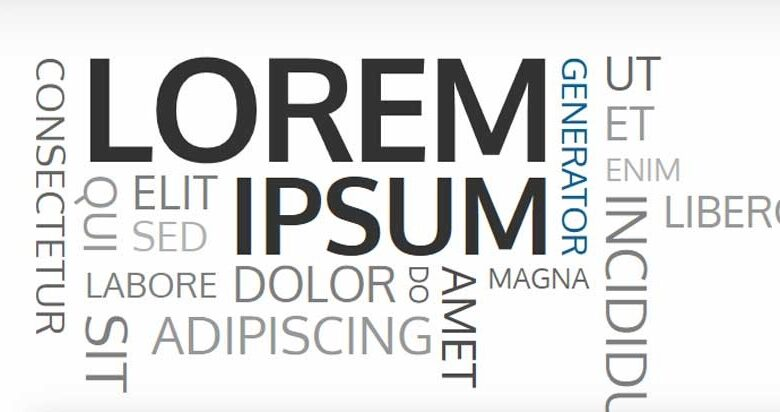
\includegraphics[width=0.5\linewidth]{Imagens/chap01/loren-ipsum-cover.jpg}
    \caption{Maecenas viverra convallis sem, id imperdiet neque rhoncus et. Ut vel mi erat. Nam quam arcu, mollis sodales felis at, sagittis iaculis lectus.}
    \label{fig:lorem_ipsum}
\end{figure}

\section{Organização do TCC}

In ornare, enim non porta interdum no Capítulo \ref{chap2},est lorem volutpat metus, pellentesque pharetra lacus est sed lacus. Vivamus quis magna et justo mattis commodo viverra in tellus. (Apêndice \ref{apendice}).

Aliquam convallis mauris sit amet elementum condimentum. Vestibulum eget tellus massa. Aenean nisl tortor, consequat ac lacus maximus, hendrerit consequat purus. Fusce aliquam, leo vel dictum molestie, lorem nibh aliquam diam, sit amet accumsan justo ante sit amet tellus no Capítulo \ref{chap6}.